% \documentclass[9pt,oneside]{amsart}
\documentclass{article}
\usepackage{xurl}
\usepackage{cancel}
\usepackage{xspace}
\usepackage{graphicx}
\usepackage{multicol,caption}
\usepackage{subfig}
\usepackage{amsmath}
\usepackage{amssymb}
\usepackage[a4paper,width=170mm,top=18mm,bottom=22mm,includeheadfoot]{geometry}
\usepackage{textcomp}
\usepackage{booktabs}
\usepackage{array}
\usepackage{verbatim}
\usepackage{caption}
\usepackage{cite}
\usepackage{float}
\usepackage{pdflscape}
\usepackage{mathtools}
\usepackage[usenames,dvipsnames]{xcolor}
\usepackage{afterpage}
\usepackage{multido}
\usepackage{color}
\usepackage{hyperref}
\usepackage{algorithm2e} % Required for pseudo-code
\usepackage{tabularx}
\graphicspath{{figs/}}
\newenvironment{Figure}
  {\par\medskip\noindent\minipage{\linewidth}}
  {\endminipage\par\medskip}

\PassOptionsToPackage{hyphens}{url}\usepackage{hyperref}
\unitlength=1mm

\providecommand{\tightlist}{%
  \setlength{\itemsep}{0pt}\setlength{\parskip}{0pt}}
 
\DeclarePairedDelimiter{\ceil}{\lceil}{\rceil}
\newcommand*\eg{e.g.\@\xspace}
\newcommand*\Eg{e.g.\@\xspace}
\newcommand*\ie{i.e.\@\xspace}
\newcommand{\fig}[1]{Figure \ref{#1}}
\newcommand{\bref}[1]{(\ref{#1})}
\newcommand{\be}{\begin{equation}}
\newcommand{\ee}{\end{equation}}
\newcommand{\bea}{\begin{eqnarray}}
\newcommand{\eea}{\end{eqnarray}}
\newcommand{\nn}{\nonumber \\}
\def\espai{\;\;\;\;\;\;\;}

\title{LAOS: Vision for a Scalable, Truly Non-Custodial,\\Dynamic NFT Protocol with Universal Minting \& Evolution }
\author{
  Alessandro Siniscalchi,
  Toni Mateos, PhD\footnote{PhD in String Theory, University of Barcelona \& Imperial College of London.}
  $ $ and Alun Evans, PhD\footnote{PhD in Medical Physics, University College London.}
  \\
  Co-Founders @ Freeverse \& LAOS \\
  \{alessandro, toni, alun\}@freeverse.io
}
\date{May, 2023}



\begin{document}

\maketitle

\begin{abstract}

This whitepaper presents the vision and design for LAOS,
a truly non-custodial dynamic NFT protocol
that, leveraging its core features of bridgeless connectivity to all EVM chains,
as well as second-order type of scalability,
aims to establish itself as the consensus system that every other
chain uses to scale their Digital Ownership transactions,
instantly and securely, and without bridging.
% 
With an architecture planned for sharding-based scalability patterns,
LAOS will enable currently mature ecosystems, such as Ethereum, to support applications
that unlock the full power of digital ownership,
migrating from the current mindset of scarcity and speculation, 
to one of abundance and captured User Generated Value.
% 
LAOS addresses the growing issue of custodianship,
where companies hold users' NFT essential data
to achieve asset mutability, thus assuming risks typically associated with securities,
by providing a genuinely decentralized legislation-compliant solution.

\end{abstract}
    


\setlength{\columnsep}{20pt}
\begin{multicols}{2}

\section{Overview}\label{overview}

LAOS, the Living Assets Open System,
aims at providing the universal platform where dynamic NFTs are created and evolved for all blockchains
in a truly non-custodial way, in contrast to highly centralized practices common today.
It will introduce and leverage the powerful concept of bridgeless minting and evolution, 
whereby developers can benefit from the features of LAOS while using any blockchain of their choice
to do trading and use DeFi services as usual, with no bridges required.

LAOS will enable DApp developers to build applications that unlock the full power of 
digital ownership, migrating from the common mindset of extreme {\it scarcity} and associated {\it speculative dynamics}, 
to one of {\it abundance} and captured {\it User Generated Value} (UGV).

LAOS will be a fully open layer 1 blockchain, decentralized via usage of its own native utility token,
built as a specialized Parachain in the Polkadot
ecosystem, inheriting its security and advanced features, and with an architecture
designed to scale as usage grows. Within Polkadot, it will leverage its trustless connection
to other Parachains specialized in smart contracts, such as Moonbeam and Astar,
and data storage, such as Crust Network.

LAOS is committed to raising public awareness about the potential risks of centralized flows
and partnering with regulatory bodies to ensure that blockchain-based
digital ownership lives up to its promise; assets that are tradable
for real money and held in privately-owned servers entail
risks akin to those typically associated with securities.

Section \ref{introduction} provides an introduction to the current landscape of NFT technology,
focusing on some of the main issues that have led to limited use cases, and highly centralized
practices. 
Section \ref{living-assets} introduces the main aspects and enabled use cases around
Living Assets.
%
Section \ref{sec:architecture} provides an in-depth walkthrough of the core 
technology and architecture of LAOS, as well as the main actors involved and their incentives.
Section \ref{sec:bridgeless-tech} describes the patterns that allow LAOS to implement
bridgeless minting and evolution. 
%
Section \ref{security} presents an analysis of attack vectors and their
potential mitigation. 
%
Section \ref{conclusion} concludes with a summary
of the main aspects presented.
\section{Current NFT Landscape}\label{introduction}

\subsection{Scalability and Use-Cases}\label{current-nfts}

During 2017, blockchain-based Non-Fungible Tokens (NFT) became popular within the crypto 
community, especially after the initial success of Cryptokitties (CK) \cite{kitties-contract}. 
CK and its successors largely set the mindset of the first wave of 
NFT-based applications; it is therefore important to understand the technical limitations that these
had to put up with.

Despite the fact that, compared to non-blockchain games, CK was an extremely limited game,
with only a handful of actions available to users, which were often executed within days of separation,
it managed to collapse the underlying Ethereum blockchain
\cite{buterin2013whitepaper}, \cite{jiang2021cryptokitties}, \cite{kitties-kraken}
when peaking around
15K daily active addresses, accounting for 25\% of all Ethereum transactions.
Fast forwarding 5 years, another game, Sunflower Farmers, reached a 40\% quota of all
gas consumed by Polygon, a scaling layer-2 on top of Ethereum, with roughly 5x more activity 
\cite{sunflower-play2earn}, \cite{sunflower-coindesk}.

These severe scalability limitations inevitably impacted on the use cases initially
implemented by different industries. On the one hand, {\it extreme scarcity} became the most exploited
pattern, since minting and trading require on-chain usage\cite{chohan2021non}.
While prices of real-world products necessarily derive from their production and
distribution costs, the price of the first wave of blockchain digital items was largely
unrelated to such costs. Artificial digital scarcity was used to increase initial selling
price, and led to purchasers {\it speculating} on 
the possibility of reselling the same item for a greater profit
(see \cite{pinto2022nft} for an interesting mathematical analysis on the expectation
of profits during the first wave of NFTs).

\subsection{Mutability and Centralization}\label{tokenURI}

Another pattern that arose due to lack of scalability was that of considering NFTs as
either {\it static} collectibles or as fully centralized digital goods; indeed, in many cases,
as both. This pattern was initiated with the rapid adoption of the ERC721 standard
\cite{erc721}, which contains an {\it optional} method
that returns a Universal Resource Identifier (URI) for every token:
\be \label{eq:tokenURI}
\mbox{tokenURI:} \mbox{ tokenId} \rightarrow \mbox{string}
\ee 
\noindent The standard suggested the following use: "This allows your smart contract to be interrogated [...] for details about the assets which your NFTs represent".

While other methods in the ERC721 standard, such as {\it ownerOf}, allow the blockchain to be
queried about {\it who owns} an asset, the optional {\it tokenURI} method aims at
being queried about {\it what is owned}. 

The vast majority of DApps ended up choosing one of the following approaches:
\bea
\label{eq:tokenURIIPFS}
\mbox{tokenURI:} \mbox{ tokenId} &\rightarrow & \mbox{IPFS address} 
\\
\label{eq:tokenURICentral}
\mbox{tokenURI:} \mbox{ tokenId} &\rightarrow &\mbox{private URL} 
\eea 

The first choice \bref{eq:tokenURIIPFS} is often made for static, immutable,
NFTs that represent assets of high value; a representative example is Beeple's
{\it Everydays—The First 5,000 Days}\cite{beeple}, sold at Christie’s for \$69.3M \cite{kugler2021non}.
In this case, the answer to {\it what is owned} refers users to the Inter-Planetary
Filesystem (IPFS \cite{benet2014ipfs}), which has the following two essential properties:
\begin{itemize}
    \item it is a {\it content addressed} system, whereby the address of a digital file
    is the result of applying a certain Hash function $H$: {IPFS address = $H$(content)};
    \item it is decentralized in nature, due to its peer-to-peer protocol.
\end{itemize}
When using the IPFS pattern \bref{eq:tokenURIIPFS}, the first property ensures that the blockchain 
returns an address that uniquely describes the content of the NFT. Together with the 
second property, the result is that {\it what is owned} can be answered in a fully 
trustless manner, without the need to query any trusted 3rd party.

The downside of pattern \bref{eq:tokenURIIPFS} is that it leads to a clash between asset 
mutability and scalability. Since any minor change in the asset's
content would necessarily map it to a different IPFS address, an 
on-chain transaction would need to be used on every change of every asset. 
Thus, pattern \bref{eq:tokenURIIPFS} is mostly used for immutable NFTs.

The centralized pattern \bref{eq:tokenURICentral} has been the choice for many DApps,
especially those that required some degree of asset mutability.
It allows developers to minimize the use
of the blockchain, by simply storing a link to external, privately-owned URLs, which
host {\it what is owned}, the asset metadata. A representative example 
is Sorare \cite{sorare},
a popular web3-based sports fantasy game, where the data of the NFTs
is stored in the company's private servers\footnote{As a concrete example, at the time of writing,
the blockchain method {\it tokenURI} for a Lionel Messi NFT \cite{messiOpenSea} pointed to
this Sorare's owned URL \cite{messiOnSorare}}

With the centralized pattern \bref{eq:tokenURICentral}, mutability is simply achieved by changing the data
provided by each company's private servers. This has several drawbacks. The most important
consequence is a critical loss of the core principles
of blockchain technology, as users must rely on private companies
for an understanding of their own holdings, thereby undermining decentralization.
Furthermore, these companies can change such data without leaving any trace, to the extreme 
of making it unavailable. Such events can even happen involuntarily, for example, 
via hacks, or because a company ceases operations, or is forced to. 
Private companies become the custodian of the attributes, and by extension,
the value of the NFT, and assume the risks associated to it. 
We shall refer to this particular highly centralized practice as the {\it elephant in the room}.

\subsection{Insecure Bridges}\label{bridges}

Finally, the aforementioned limitations have also forced DApp developers 
to make undesired compromises when selecting the blockchain to build on.
Concerns around gas costs, availability of the underlying coin, user base 
of the existing DeFi ecosystem, or degree of decentralization and
security are weighted against the needs of each specific application.

Bridges are often built to allow users to migrate assets across blockchains,
which tends to be a complex UX process.
But building bridges is hard. Almost every relevant
bridge built to date requires some level of centralization,
and many of them have been hacked\cite{lee2022sok},
resulting in millions of stolen funds. Examples include
widely used bridges between Ethereum and Solana\cite{eth-solana},
bridges required to play {\it Axie Infinity},
the most popular NFT-based game at the time\cite{axie-bridge-1}, \cite{axie-bridge-2},
as well as vulnerabilities of up to \$850M that 
were live for some time in the Polygon to Ethereum bridge,
but fixed before being exploited\cite{polygon-hack}.


\subsection{Growing Legal Concerns}\label{summary}

As discussed, initial limitations of fully programmable-blockchain technology
led to many of the early NFT use cases relying on some combination of
extreme scarcity and speculation, making choices between an immutable approach, 
or highly centralized practices, and often forcing users to go through insecure bridges.

Legislation is indeed starting to pay closer attention to centralized NFT flows. A relevant
example is the recent class-action lawsuit filed against the popular NFT-based application 
NBA Top Shot\cite{nba}, to decide whether or not their NFTs should be considered
unregistered securities\cite{dapper-labs-nft-ruling}. Although this lawsuit 
does not deal with the {\it elephant in the room} directly, the judge 
did argue that users were forced to rely on the running of the platform by a few
private actors,
leading to {\it expectation of profit being “derived from the efforts of others”}.

Although legislation in the web3 space is a highly complex, rapidly evolving field,
it may well be the case that similar NFT-as-securities lawsuits follow soon, 
given the aforementioned custodian role that many private companies are currently assuming. 




\section{Living Assets and LAOS}\label{living-assets}

Living Assets (LA) are Non-Fungible Tokens implemented in LAOS. 
LA extend the technology of the first wave of NFT by adding the
following features:
\begin{itemize}
    \item Scalability. LA can evolve at scale, in fully decentralized flows;
    \item Full Decentralization. The attributes of all LA, now, and in every past state, can be certified on-chain, without 
    resorting to centralized privately-owned servers (technical details in Section \ref{sec:architecture});
    \item Bridgeless Minting \& Evolution. LA can be traded in any blockchain that supports smart contracts,
    while being minted and evolved in LAOS, without the need to resort to any type of bridge
    (technical details in Section \ref{sec:bridgeless-tech}).
\end{itemize}

The following subsections provide a high-level overview of how these 
properties can be leveraged, focusing on the developers and users
point of view. The low-level technical
aspects are left for sections \ref{sec:architecture} and  \ref{sec:bridgeless-tech}.

\subsection{User Generated Value}\label{sec:ugv}

Scalability and the trust generated by the fact that 
mutability has a fully verifiable history are the key ingredients 
to one of the main paradigm shifts that Living Assets enable.

LA enable digital industries to migrate from a mindset of {\it scarcity} and {\it speculation},
to one of {\it abundance} and {\it User Generated Value} (UGV). In the latter, 
assets can be distributed at scale, at zero or very small initial value
(e.g., just for downloading and application or for signing-in), to a large base of users, hence 
eliminating all monetary entry barriers to owning a digital asset.

In this mindset of abundance, the initial market value of most assets is effectively zero.
DApps using LA can provide the flexibility to evolve based on both
off-chain activity (such as real-world events) and on-chain data.
By engaging with apps, video games,
online and social media activity, and the broader ecosystem,
LA owners can improve their assets (a more powerful game item,
an NFT that grants better rewards, an IP license granting further rights),
making them more valuable to others,
eventually converting their dedication, talent, and effort,
into increased market value.

\begin{Figure}
    \medskip
    
\includegraphics[width=1\textwidth]{pyramid.png}
    \captionof{figure}{
        Typical distribution of market value (y-axis) vs. 
        number of assets (width of the x-axis)
        in User Generated Value paradigms. A large number of assets with negligible market value 
        co-exist alongside a smaller percentage that have accrued significant value
        through the efforts of their owners.
    }
    \medskip
    \label{fig:pyramid}
\end{Figure}

UGV paradigms tend to reflect patterns common to Free-to-Play models
(Figure \ref{fig:pyramid}), whereby
a large base of assets with near-zero market value co-exist with further layers
of assets which users have evolved significantly with their actions. This pattern turns the 
sentiment of owning digital assets into an {\it active} experience, 
becoming a powerful engagement tool.


\subsection{Certifiability}\label{sec:ugv-certifiable}

UGV and the use cases mentioned in sections \ref{sec:la-bridglessness}-\ref{sec:use cases}
heavily rely on the history of the asset, on the confidence that NFTs have
market value accrued through a fair, traceable, set of evolutions.
It becomes paramount to be able to answer, in a fully trustless way, 
questions like {\it how did users turn this game item into something so powerful?}, or {\it how did
the owners of this NFT evolve it from scratch to an item with level-10 rewards?}

This is manifestly impossible in centralized flows derived from 
pattern \bref{eq:tokenURICentral}, since external privately-owned servers need 
to be trusted, exactly as in the pre-blockchain era.

LAOS provides the strongest forms of certifiability. On the one hand,
as described in Section \ref{sec:architecture}, all {\it data is fully available}
via decentralized flows, including data about the current and
past attributes of every asset.

On the other hand, LAOS enables any party to prove on-chain that an asset
with tokenId $id$ was in a certain state $s$ at any time $t$ in its history,
via the provision
of inclusion proofs $\Pi(id, s,t)$; these allow the blockchain to build {\it verify} 
methods which return true/false when queried:
\bea
\mbox{verify: \espai} id, s, t, \Pi(id, s,t) & \rightarrow & \mbox{bool}\,.
\eea

By virtue of LAOS being in the Polkadot ecosystem, it will be possible
to use these strong forms of certifiability as part of smart contract logic
built in other Parachains, such as Moonbeam\cite{moonbeam} or Astar\cite{astar}.
Example use cases would be contracts that allow owners of 
NFTs that have been evolved beyond a certain level to unlock certain rewards,
or that execute methods of a DeFi contract in the same blockchain.
An illustrative example of pseudo-code would be:
\begin{algorithm}[H]
    \KwData{Input values $id, s, t, \Pi(id, s,t)$}
    do initial logic\;
    \If{\textnormal{verify($id, s, t, \Pi$($id, s,t$))}}{
        do further logic based on $s,t$\;
    }
\end{algorithm}

Perhaps the simplest, yet powerful, example of this usage would be to enable {\it certified purchases}.
In this pattern, a buyer could sign a purchase transaction that is conditional on the asset
attributes, e.g., "buy this asset if and only if it has {\it level} larger than 100".

\subsection{Bridgeless Minting \& Evolution}\label{sec:la-bridglessness}

The scalable, strongly-certifiable, minting and evolution features of LAOS
can be added on top of the advantages that leading blockchains already
have in terms of mature ecosystems of users and DApps.

By means of example, we hereby discuss the use case of developers that
want to build applications which benefit both from LAOS features and
Ethereum's rich ecosystem of smart contracts and DApps.
Any other blockchain that supports Turing-complete
programming of smart contracts would work too. 

Developers only need to deploy once
an ERC721/1155 smart contract in Ethereum,
tuned to use the Universal Location pattern as described
in section \ref{sec:bridgeless-tech}. Next, they can mint and evolve
assets in that contract by simply executing the corresponding transactions in the 
LAOS blockchain. Anyone can permissionlessly, in a fully decentralized manner,
and without resorting to bridges, build new, or connect to existing,
marketplaces that operate with these assets by means of standard
ERC721/1155 calls on Ethereum.
In particular, this contract's assets can be connected, e.g., to smart contracts
in Ethereum that allow their rental or to fractionalize their ownership.

By doing so, applications can leverage paradigms where massive amounts
of assets are created in a scalable, certifiable way, in LAOS, with only
a small fraction of them having fairly accrued enough User Generated Value 
to be worth tradeable in Ethereum.


\subsection{Use cases}\label{sec:use cases}

Living Assets profoundly change traditional paradigms,
heralding new prospects for creators, users, and industries at large.
By actively engaging with LA, owners wield the power
to shape and influence the attributes of their assets,
thereby directly impacting their intrinsic value.
This interactive participation fosters deeper connections between
users and their assets, transcending the conventional
notion of passive ownership.

The reimagining of digital ownership opens up
a wide range of compelling use cases.
With developers and their communities empowered by
new tools and increased flexibility,
it is impossible to predict the full extent of their
creative potential. Nevertheless, here are a few examples
that can be envisaged today.

{\bf Brand Loyalty Program.}
Consider the prospect of owning a 
cool new shoe from one of the world's most admired shoe manufacturers
that undergoes progressive "leveling up" in
design and quality as a direct consequence of brand mentions,
retweets, and shares achieved by the owner on social media platforms.
This interactive paradigm unlocks escalating discounts and privileges, forging deeper bonds of loyalty and engagement with the brand.

{\bf Entertainment.}
In the realm of entertainment,
LA enable the possession
of hyperreal Avatars representing beloved celebrities.
These Avatars evolve dynamically in response
to user interactions within their ecosystem,
encompassing activities such as quizzes,
merchandise engagement, and attendance at real-world events.
As users ascend to higher levels through sustained participation,
exclusive privileges like meet-and-greet opportunities unlock.

{\bf Gaming.}
LA empowers the gaming landscape by
endowing players with the ability to nurture the evolutionary journey
of their weapons, such as an "axe,"
from rudimentary stages to lofty tiers of rarity,
namely epic and legendary.
This progression is intrinsically linked to the player's skill,
dedication, and accomplishments within the game,
creating a gratifying sense of {\it fairness}, achievement and recognition.

{\bf Intellectual Property (IP) Rights.}
LA introduce innovative possibilities for the
dynamic evolution of IP licenses
associated with digital artwork.
At the outset, the license may impose stringent restrictions,
confining the permissible print size to dimensions no larger than A4.
However, as users proactively promote the artist and acquire
additional pieces from the artist's collection,
the license undergoes an evolutionary transformation.
Ultimately, it may grant permission for the artwork to be exhibited for-profit,
including the prerogative to levy an entrance fee.
This seamless evolution is intricately encoded within the asset's
attributes, ensuring transparency, integrity, and equitable governance.

{\bf User Generated Content.}
LA allows the flourishing community of content generators to 
accrue market value to their talent and dedication. In an in-game example,
users can customize their in-game racing car,
from engine tweaks, to paint job and looks,
making it drive faster and look awesome,
and be more desirable for every other player.




\section{Architecture}\label{sec:architecture}

The architecture of LAOS is discussed in detail in
Section \ref{sec:arch-highlevel}, after an initial
discussion of a key separation pattern of asset ownership 
and asset attributes used all across LAOS in Section \ref{sec:separation}.
Section \ref{sec:architecture-future}
concludes with the vision beyond the initial implementation.


\subsection{The Ownership-Attributes Split}\label{sec:separation}

At the core of the technology is a hard separation
between asset ownership and asset attributes, brought to the extreme
whereby both sets of data can live and be managed by different blockchains,
but carefully designed to be properly linked, 
and allow for on-chain traceability and certification.

Unlike traditional NFTs, where both sets are either stored on-chain
in the same blockchain's contract, or where the attributes are stored
in external, static, content-addressed systems (pattern \bref{eq:tokenURIIPFS})
or in external, privately-owned servers (pattern \bref{eq:tokenURICentral}),
LAOS separation allows both sets of data to live in different decentralized {\it 
consensus systems}.

\begin{Figure}
    \medskip
    
\includegraphics[width=1\textwidth]{patterns.png}
    \captionof{figure}{
        Typical structure of nodes/services required to run a DApp, such as a marketplace:
        (a) a consensus node, e.g., an Ethereum node; (b)
        an IPFS node, for NFTs implementing pattern \bref{eq:tokenURIIPFS}; (c)
        access to privately-owned internet servers, for NFTs implementing pattern \bref{eq:tokenURICentral}.
    }
    \medskip
    \label{fig:patterns}
\end{Figure}

Figure \ref{fig:patterns} illustrates the traditional NFT node structure to which
DApps normally connect. While DApp developers
have the choice to operate their own consensus nodes,
particularly for fully permissionless blockchains,
it is commonplace to rely on third-party node providers that
ensure consistent uptime and handle maintenance \cite{stogerdemystifying}.
Likewise, developers often opt to use third-party IPFS providers to guarantee 
that content is pinned with high data availability.

\begin{Figure}
    \medskip
    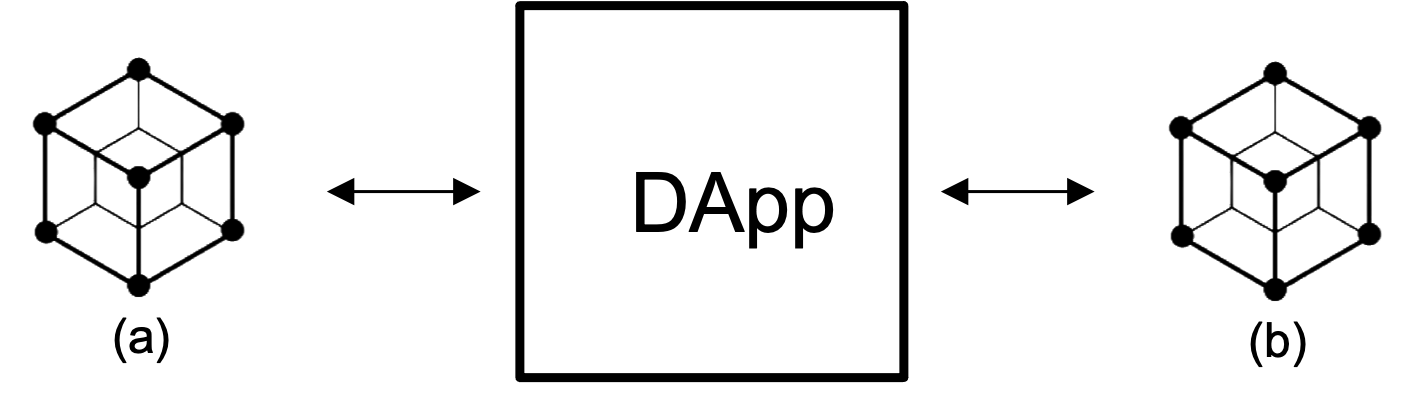
\includegraphics[width=1\textwidth]{patterns_2nodes.png}
    \captionof{figure}{
        Structure of nodes when implementing the ownership-attributes split,
        with a DApp using two different consensus nodes, one for ownership (a)
        and one for attributes (b).
    }
    \medskip
    \label{fig:patterns2nodes}
\end{Figure}

Figure \ref{fig:patterns2nodes} shows the structure for patterns
based on LAOS' ownership-attributes split, whereby only consensus nodes are
required. Figure \ref{fig:patterns2nodesAs1} shows a convenient architecture
where the DApp only interacts with one single node, which can be built permissionlessly:
the node maintains a state that internally syncs with the two consensus system,
and exposes a single API that abstracts all complexity, and mimics a single ERC721/1155
compliant system. 

\begin{Figure}
    \medskip
    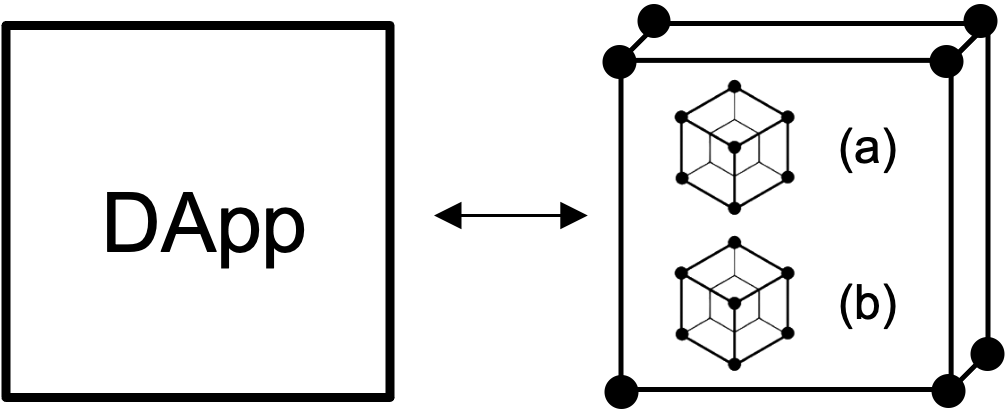
\includegraphics[width=1\textwidth]{patterns_2nodesAs1.png}
        \captionof{figure}{
            A convenient way to structure nodes in ownership-attributes split patterns,
            where a DApp interacts via the ERC721/1155 standard interface 
            with one single node that abstracts all complexity.
        }
    \medskip
    \label{fig:patterns2nodesAs1}
\end{Figure}

The link between both consensus systems can be achieved by using recently developed standards
like the {\it Universal Location} pattern, introduced as part of XCMv3 by
Polkadot, and described in more detailed in section \ref{sec:universal-location}.
From the point of view of the patterns described in section \ref{tokenURI},
this standard enables the DApps to reference assets that live in different
consensus systems:
\bea
\label{eq:tokenURIConsensus}
\mbox{tokenURI:} \mbox{ tokenId} &\rightarrow & \mbox{Consensus Address} 
\eea 

This fundamental aspect, as well as the design to link both systems,
is reflected the LAOS architecture detailed in the next
sections, and sits at the core of the bridgeless minting \& evolution feature
discussed in Section \ref{sec:bridgeless-tech}.

\subsection{High-level architecture}\label{sec:arch-highlevel}


\subsubsection{Leveraging Polkadot's ecosystem and features}

LAOS is architected as a specialized Parachain in Polkadot\cite{polkadot}, \cite{polkadotExplained},
fully devoted to providing the ideal platform to fulfill the aforementioned requirements and vision.
The architectural design choices exploit several benefits that are unique to Polkadot, among others:
\begin{itemize}
    \item as a Parachain, it will automatically inherit the full security guarantees 
    provided by Polkadot's Relay Chain from day 1;
    \item by internally being built on Substrate and using the GRANDPA\footnote{GRANDPA stands for GHOST-based Recursive Ancestor Deriving Prefix Agreement, a finality gadget for consensus systems originally presented in\cite{grandpa}.}
    consensus algorithm, it will also share top features such as non-probabilistic
    fast block finality, and forkless upgrades of its protocol;
    \item it will make use of Polkadot's recently introduced Universal Location pattern, as part of XCMv3;
    \item it will heavily leverage other Parachains in the ecosystem, making it easy to interact
    with EVM-compatible smart contracts, guarantee long-term data availability, access to DeFi, and
    benefitting from a combined maximum transactions per second (TPS) estimated between 100K and 1M;
    \item it will allow its internal design to leverage Polkadot's developed Relay Chain 
    and trustless bridges technology to achieve, mid-term, a scalability comparable to second order relay chains.   
\end{itemize}

As side benefits, Polkadot's available rich set of tools and open code bases will
allow LAOS to avoid reinventing the wheel, use battle-tested software,
and progressively adopt upgrades developed by other teams, while contributing to the ecosystem.

\subsubsection{Components}

LAOS will by built around the architecture depicted in \fig{fig:architecture}.
We hereby detail its main system components.

\begin{Figure}
    \medskip
    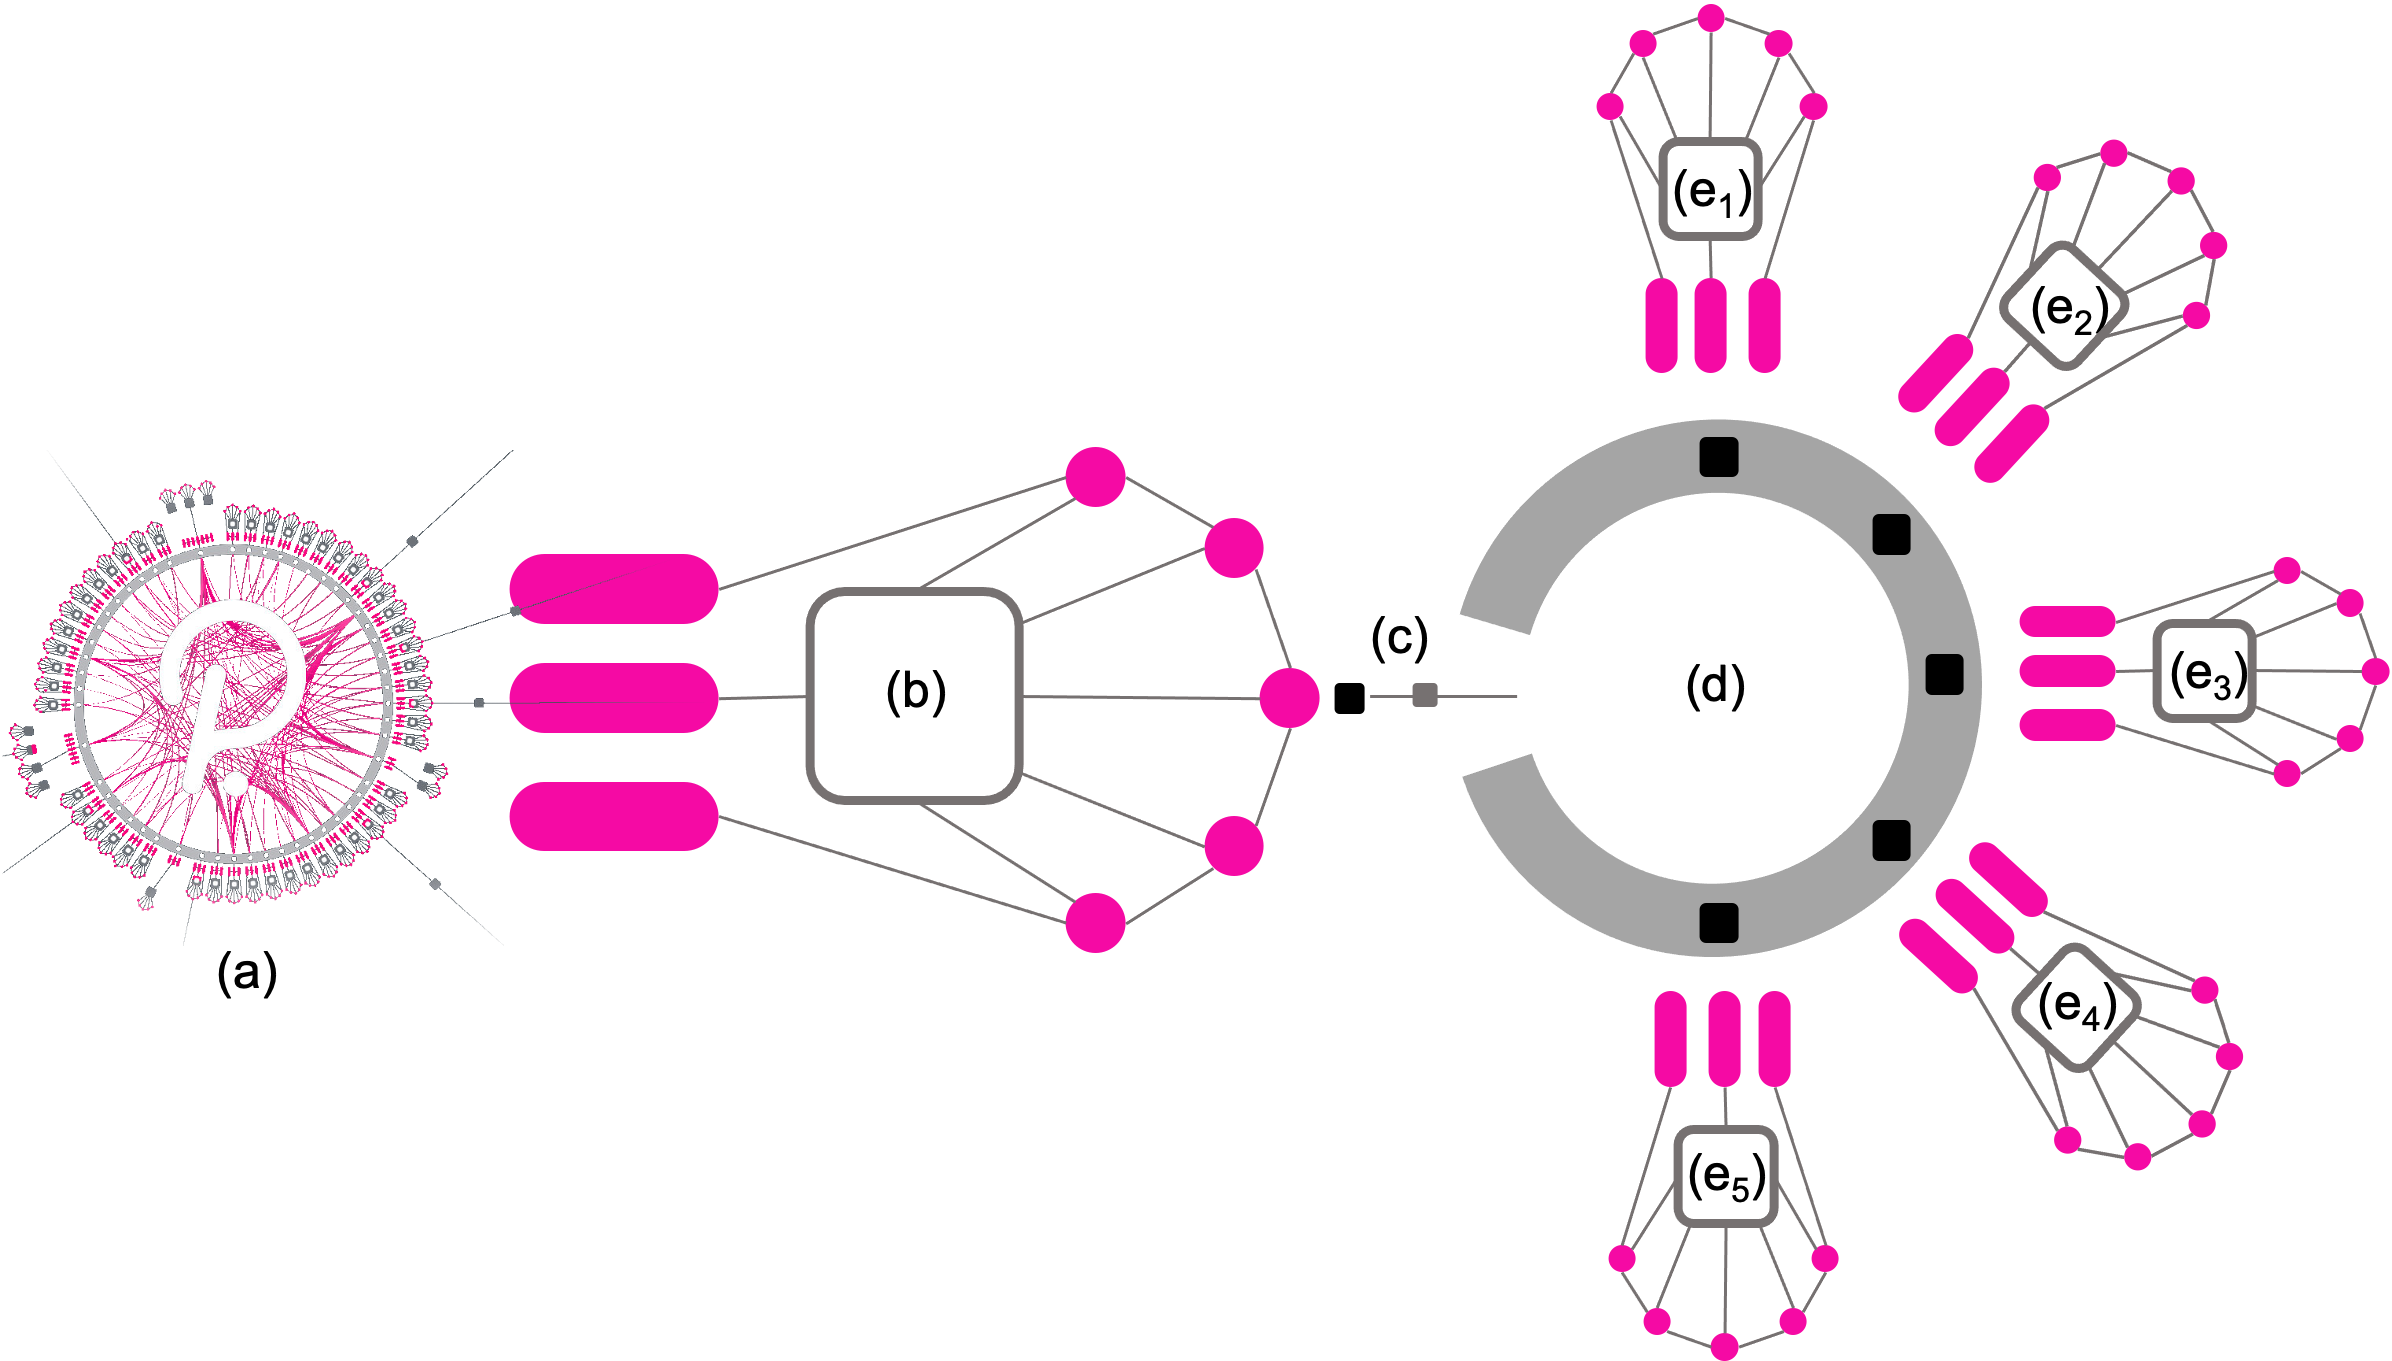
\includegraphics[width=1\textwidth]{laos-architecture.png}
        \captionof{figure}{
            Vision for the core design of LAOS: the LAOS Relay Chain (d)
            is connected to the Ownership Parachain (b)
            via one single trustless bridge (c),
            while its set of validators provide security
            to the Evochains (e$_i$) via the standard Polkadot
            Relay Chain to Parachain sharding pattern.
        }
    \medskip
    \label{fig:architecture}
\end{Figure}

\vspace{\baselineskip}

{\bf (a) Polkadot's Relay Chain.}
At the root of the LAOS consensus protocol is Polkadot's Relay Chain, with the set 
of Polkadot validators that provide security to the Parachain, ensuring that
every transaction processed by a Parachain is valid. The Relay Chain
also help Parachains transfer assets and connect functionalities in a fully
trustless way via native Cross-Consensus Messaging (XCM), efficiently 
linking the light clients that Parachains have from other Parachains.

\vspace{\baselineskip}

{\bf (b) LAOS Ownership Parachain.}
The LAOS Ownership Parachain will be a specialized chain, based on the 
Polkadot standard NPoS protocol, with the following functionalities:
\begin{itemize}
    \item host and manage the LAOS native utility token;
    \item manage the ownership of all LA created directly in LAOS, with 
    transactions implemented at the protocol level,
    and fees paid in the native tokens;
    \item manage runtime upgrades of LAOS' Relay Chain, and all Evolution Chains (Evochains);
    \item store state roots of the Evochains, exposing asset attributes
    certification methods,
    and reward LAOS Relay Chain validators upon reception of new correct roots;
    \item manage all trustless transfers of LAOS Assets and LAOS tokens
    between LAOS and the rest of Parachains via XCM;
    \item implement and coordinate governance and staking.
\end{itemize}

\vspace{\baselineskip}

{\bf (c) GRANDPA-Based Trustless Bridge.}
LAOS will make use of the bridge technology developed 
by Polkadot ecosystem to trustlessly connect Substrate-based 
chains with GRANDPA finality\cite{parity-bridges},
which is expected to connect, among others,
Polkadot and Kusama via BridgeHub\cite{bridgehub}.

The security of this bridge design relies on each chain's set of validators
running a light client of the other chain; this enables each endpoint to     
mathematically verify any statement received about 
the state of the other chain. In particular, new headers are accepted only
after verification of the required majority of validators of the other chain.

The bridge will be used to teleport LAOS tokens among the Ownership, LAOS Relay Chain,
and the Evochains, always with a 1:1 parity, to enable payments of gas fees for 
mint and evolve transactions, irrespective of whether they corresponds
to assets that can be traded in the LAOS Parachain, or in other
blockchains via remote, bridgeless minting and evolution.

Likewise, the bridge will be used to constantly record the state of the LAOS Relay Chain,
and its Evochains, in the LAOS Ownership Parachain, allowing on-chain verification of all assets
attributes, including every state they went through.

\vspace{\baselineskip}

{\bf (d) LAOS Relay Chain.}
Connected to the Ownership Parachain via one single trustless bridge (c),
and providing security to the Evochains (e$_i$) sits a specialized, limited-functionality,
version of
Polkadot's Relay Chain. Both chains at the end of the bridge run a light-client
of each other, ensuring that their full states are mutually known in a permissionless
way.  

The LAOS Relay Chain runtime upgrades are orchestrated by
the Ownership chain via XCM commands across the trustless bridge.
Likewise, this Relay Chain will not have a native token; it's economy will use 
LAOS tokens reserve transferred from the the Ownership Parachain.

In turn the LAOS Relay Chain will provide security to its Parachains following exactly
the same pattern as Polkadot's Relay Chain.

\vspace{\baselineskip}

{\bf (e) LAOS Evochains.}
LAOS Assets are created and evolved in the Evochains.
They are Parachains of the LAOS Relay Chain,
supporting asset mint and evolution at protocol level.

All Evochains share the same runtime, and runtime upgrades are orchestrated by the
LAOS Relay Chain, the runtime of which is in turn orchestrated by the Ownership Parachain.
Similarly, Evochains do not have a native token. DApp developers that create  
and evolve LA pay transaction fees to Evochain collators in teleported LAOS tokens.

Each Evochain supports a large number of DApps, and new Evochains are spawned when approaching full capacity,
as opposed to simply increasing gas price. When Polkadot Parathreads and on-demand patterns
are fully consolidated, LAOS will consider integrating them as an additional complementary pattern. 

Note that the trustless bridge ensures that the state of every Evochain
remains in the Ownership Parachain, allowing for certification of
every attribute of every LA, via standard Merkle proofs.


\subsection{Scalability} \label{sec:architecture-future}

The described architecture does not attempt to reproduce  
a {\it Polkadot-inside-Polkadot} 2nd-order-relay pattern, but rather,
to constitute a specialized system, focusing on scaling homogeneously,
supporting Evochains managed by exactly the same runtime.  

As usage grows, LAOS stands to benefit directly from
Polkadot's sharding technology, which enables the spawning of
new Evochains, while maintaining their security through a single set of validators.

LAOS overall throughput, typically measured in transactions per second,
is expected to align with Polkadot's own estimates as the combined throughput
for all its Parachains. 
\section{Bridgeless Minting \& Evolution}\label{sec:bridgeless-tech}

The architecture described in section \ref{sec:architecture} supports 
a pattern capable of enabling the minting and evolution
of assets in LAOS, while their trading (and any other ownership-related
concept) is managed in any other blockchain of choice, as 
long as it supports smart contracts; this applies to both EVM and
non-EVM compatible cases. We stress that this does not require any
type of bridge, neither trusted nor trustless.

We first introduce the concept of
Universal Location in Section \ref{sec:universal-location},
and then describe a simplified version of the pattern which 
only allows bridgeless evolution (Section \ref{sec:bridgless-evo}).
We conclude discussing the full-fledged flow for bridgeless minting and evolution
in Section \ref{sec:bridgless-all}.

\subsection{Universal Location}\label{sec:universal-location}

One recent standard that LAOS will leverage is that of {\it Universal
Location}. It was introduced by Polkadot as a natural evolution
of the {\it MultiLocation} standard that was already in use within their
ecosystem, as part of their Cross-Consensus Messaging (XCM)
pattern\cite{multilocation}.

The fact that the Relay Chain serves as consensus parent for all
Parachains has enabled the design of trustless message-passing patterns
among Parachains, for example, by relying on the light clients
that collators of Parachains have from other Parachains.

MultiLocation assists this communication by identifying
every single location that exists within the world of consensus
systems that share a common parent, and example being all Parachains,
as their finality derives from the consensus in the parent Relay Chain.
A location in a consensus system is defined as an
{\it isolatable state machine} held within global consensus.

For instance, the following:

\begin{align}
    & \text{MultiLocation =}  \label{eq:multilocation1} \\
    & \,\, ../\text{Parachain}(42)/\text{AccountKey20}(0x12...cd) \nonumber
\end{align}

can be used by one Parachain to refer to a 20-byte account ($0x12...cd$)
that exists within a different Parachain (42), that shares the same parent consensus
system: the Relay Chain (at '$../$').

By contrast, Polkadot's XCMv3\cite{multilocationXCMv3} introduced 
the concept of a {\it Universal Location} under which all systems
which generate their own consensus exist, and by extension,
all possible locations within consensus. The Universal Location is the only location
that has no parent. In typical filesystem formatting, the Universal Location 
can be thought of as the {\it root},
often represented by the starting '$/$' symbol of a path.

Universal Location enables the creation of routes that
connect smart contracts in an origin blockchain
to assets or accounts in, e.g., Polkadot, through references such as:
\begin{align}
     & \text{MultiLocation =}  \label{eq:multilocation2} \\
     & \,\, /\text{Polkadot}/\text{Parachain}(42)/\text{AccountKey20}(0x12...cd) \nonumber
\end{align}

Finally, the {\it MultiAsset} part of the standard uses these concepts to
standardize the referral to both fungible and non-fungible tokens.

\subsection{Bridgeless Evolution}\label{sec:bridgless-evo}

The simplest usage of LAOS for developers that want the
ownership of assets to be managed by a different blockchain, e.g., Ethereum,
is to simply mint assets in the origin blockchain, and 
use a LAOS MultiLocation string, using the Universal Location '$/$' as root,
to specify the tokenURI, 
effectively using \bref{eq:multilocation2} to create a concrete implementation
of pattern \bref{eq:tokenURIConsensus}:
\bea
\mbox{tokenURI:} \mbox{ tokenId} &\rightarrow & \mbox{LAOS MultiLocation}
\nn 
\label{eq:tokenURILaos}
\eea 
As Figure \ref{fig:patterns2nodesAs1} depicts, all that DApps need 
to build applications that use this pattern 
is to query a LAOS node to resolve tokenURIs and provide asset metadata.

This pattern basically links the asset metadata to an updatable slot governed
by a consensus system, with transparency, traceability,
data availability for both current 
and past states. And it does so in a flow which, ultimately, does not require of 
any trusted party.

In this pattern, however, asset minting is still required in the origin
blockchain, potentially running into scalability issues or incurring 
in high gas prices. 

\subsection{Bridgeless Minting \& Evolution}\label{sec:bridgless-all}

The previous pattern becomes more powerful when {\it minting} of assets,
as opposed to only evolution, can also be offloaded to LAOS by any 
other blockchain. We shall first discuss the nomenclature and 
the building blocks required to build this functionality, and then
analyze the resulting flow.

This process requires two simple components: a pattern to build the {\it id} 
of assets, and a piece of smart contract logic that utilizes the meaning
that can be extracted from such {\it ids}.  

\subsubsection{Encoding \& Decoding Methods}
The setup starts with the usage of a concrete pattern to
generate {\it ids} for assets, enabling the encoding of a
generic web3 address ({\it w3a}). Let us call $Enc$ and $Dec$ the encoding
and decoding functions, correspondingly:
\bea
Enc: & w3a, \Omega & \rightarrow id \,,
\nn
Dec: & id  & \rightarrow w3a\,,
\label{eq:enc-dec}
\eea
where $\Omega$ represents any other information that the {\it id} may
contain, e.g., a consecutive index often used to distinguish assets as they
are minted. 

$Enc$ is an injective function; in particular, two assets with different {\it id} must 
necessarily differ in either $w3a$ or $\Omega$. Note, however, that there may be
a large number of assets that share the same $w3a$, as made manifest
by the $Dec$ function, which projects out all information conveyed by $\Omega$.

A simple example for an $Enc$ function is provided by the binary concatenation of 
the binary representations of $w3a$ and $\Omega$, which corresponds to a sibling
$Dec$ function that trims the bits assigned to $w3a$.

\subsubsection{Smart Contract Logic}
The ERC721/1155 smart contract logic required in the origin blockchain must 
contain a minor code extension in the implementation of the 
$ownerOf$ (and related) methods. 

For the sake of simplicity, let us assume that the smart contract implements 
a simple method, $localStorage.wasEverTraded(id)$, that returns {\it true} if the asset 
has been traded {\it at least once}. On deploy of the smart contract,
this method naturally returns $false$ for every $id$.

As customary, the contract writes to storage as assets are traded,
allowing a method we shall call {\it localStorage.ownerOf} to return
the new owners, and reflecting in positive returns of $wasEverTraded$.
These methods can be used to extend $ownerOf$ as follows:

\begin{algorithm}[H]
    \SetKwFunction{GetOwner}{ownerOf(id)}
    \SetKwData{wasEverTraded}{localStorage.wasEverTraded(id)}
    \SetKwData{localStorage}{localStorage.ownerOf(id)}
    \SetKwData{defaultOwner}{Dec(id)}
    
    \SetKwProg{Procedure}{method}{}{}
    \Procedure{\GetOwner}{
        \If{\wasEverTraded}
        {
            \KwRet \localStorage\;
        }
        \Else{
            \KwRet \defaultOwner\;
        }
    }
\end{algorithm}

\subsubsection{Resulting Flow}

The final ingredient required for bridgeless minting is implemented in LAOS,
by simply using exactly the same encoder/decoder functions \bref{eq:enc-dec} to name assets
in the Evochains, and declaring assets in these particular collections as {\it foreign 
assets}, signalling that they cannot be traded in the LAOS Ownership Chain.

The aforementioned smart contract logic, together with the LAOS MultiLocation
pattern \bref{eq:tokenURILaos}, allows one single deploy of an ERC721/1155
contract in an origin blockchain to link all assets to LAOS, while retaining 
the management of all ownership-related aspects in the origin chain. 
In effect, all assets ever assignable to all potential initial owners are reserved on deploy,
and the LAOS consensus system is assigned the responsibility to {\it fill-in} the
corresponding initially-empty registers as assets are minted, and modify them
as they are evolved.

Again, figure \ref{fig:patterns2nodesAs1} illustrates a convenient way to architecture
nodes that would serve bridgeless minting and evolution; in this case, the ownership
node would be one of the origin chain.
 
\section{Security}\label{security}

LAOS core components are based on software and consensus protocols
that are already in use,
and analyzed extensively by other teams.
In this sense, LAOS security analysis is different from 
projects proposing entirely new, still untested, protocols;
in LAOS case, the analysis mostly consists of, for every component
in its architecture, relying on previously published
comprehensive studies of their attack vectors and potential mitigation.

\subsection{Ownership Parachain}\label{sec:security-parachain}

The Ownership Parachain will
implement the default Parachain pattern that relies on the Polkadot
Relay Chain to provide block finality \cite{parachain-protocol}, \cite{parachain-protocol2}.
This protocol enables efficient heterogeneous sharding,
and has been live in mainnet, in Kusama first, since
October'19, and then in Polkadot, since March'20.

Parachains are free to decide their runtime and are encouraged to focus on 
specialization, in contrast to the one-runtime-fits-all
homogeneous sharding being built in Ethereum 2.0.
LAOS will diligently adhere to this pattern,
specializing in all aspects relevant to Digital Ownership.
The Ownership Chain will use the default Parachain pattern:
Nominated Proof of Stake (NPoS) consensus algorithm,
with GRANDPA providing finality over BABE block production.
We refer the reader to the thorough theoretical analysis presented in\cite{polkadotExplained}
for full details.

It is essential to note that despite the freedom that Parachains have to design
their inner details, every single transaction of every Parachain is eventually
verified by the required majority of validators in the Relay Chain before
being included in a Polkadot block. 

Since the consolidation in Polkadot of Parachain's 
invalid transactions is prevented by the Relay Chain, 
the only significant attack vectors relevant to Parachains
are related to censorship and data availability.

Censorship corresponds to Parachain collators not including one or more
transactions based on criteria different from those specified by the
protocol, e.g., based on the sender address. To prevent these attacks,
a Parachain only needs to ensure that there are some neutral collators,
but not necessarily a majority.
Theoretically, the censorship problem is solved with 
having just one honest collator,
as analyzed in\cite{collators}.

Data availability attacks appear if the Parachain collators collude to 
withhold block data, or the corresponding Proof of Validity (PoV), to the 
validators in the Relay Chain. 
Polkadot's protocol mitigates this 
attack severely by using Erasure Coding\cite{al2018fraud}, which
adds redundancy on the block/PoV data 
made availability by a minimal subset of honest collators, and enables Relay Chain
validators to reconstruct its entirety out
of a small set of randomly queried data.

In summary, the standard Parachain-in-Polkadot level of security 
protects all features assigned to the Ownership Parachain,
including transfers of LAOS assets and tokens among owners as well as to
sibling Parachains, management of the LAOS token, 
transaction fees, treasury funding, storage of LAOS Relay Chain and Evochain states,
and management of their runtimes.

\subsection{Trustless Bridge}\label{sec:security-bridge}

The design of the bridge that will connect the Ownership Chain 
and the LAOS Relay Chain is built around the same technology that 
will connect Polkadot and Kusama via BridgeHub\cite{bridgehub}.

This bridge design decouples the consensus mechanism
and the state machine, requiring both networks to run 
{\it on-chain consensus clients}, also known as {\it on-chain light clients},
that only track consensus proofs of state
transitions instead of the full state transitions.
References \cite{SeunLanlege} and \cite{snowfork} provide a good introduction to 
known attack vectors to light client based bridges in systems
that either do not track the signatures of all validators, or do 
not implement accountability on validators that provide multiple signatures
over different block proposals. 

Instead, the bridge implementation is based on the on-chain light
client used by Polkadot and Kusama~\cite{parity-bridges}, 
designed only for systems whose finality is provided by the GRANDPA finality gadget.
Eventually, the bridge will become more efficient when Polkadot integrates
{\it on-chain accountable light clients}, which use signature
verification via Zero-Knowledge schemes, and introduce on-chain
accountability mechanisms. We refer the reader to~\cite{ciobotaru2022accountable}
for a thorough analysis of attack vectors.

Regarding data withholding attack vectors,
it is important to consider that any actor can 
relay block data and the corresponding transition proofs
between the Ownership Chain and the LAOS Relay Chain.
The attack can be straightforwardly mitigated by having at least one
actor with incentives in the LAOS platform running a node of the
LAOS Relay Chain, even if in read-only mode, capable of relaying 
the Evochain data as new blocks are produced.

Moreover, the LAOS Relay Chain validators have their own incentives
to relay this data because they receive rewards
in the form of LAOS tokens
upon inclusion of new valid blocks in the Ownership Chain.


\subsection{LAOS Relay Chain}\label{sec:security-laos-relay}
 
The LAOS Relay Chain is an instance of Polkadot's Substrate-based Relay Chain,
with GRANDPA finality.
As such, its security depends
on the standard game-theoretical incentive system that
leads to more than two-thirds of their validators following
the protocol honestly.

A comprehensive analysis of GRANDPA, including a listing of 
attack vectors and their potential mitigation, can be found in\cite{grandpa}.

LAOS Relay Chain validators will be rewarded for including valid blocks
from the Evochains, through transaction fees in LAOS tokens obtained from
the Ownership Chain via the trustless bridge. Likewise, they will be rewarded
when new block headers of the LAOS Relay Chain are correctly included in the Ownership Chain,
in this case, in native LAOS tokens. 
This incentive system encourages LAOS Relay Chain validators
to not only provide data to the bridge relayers
but also potentially take on the role of bridge relayers themselves.

\subsection{Evochains}\label{sec:security-evochains}

Evochains are Parachains of the LAOS Relay Chain,
supporting asset mint and evolution at protocol level.
As such, the same security considerations discussed for the Ownership Parachains
(Section ~\ref{sec:security-parachain}) apply to the Evochains, replacing
Polkadot's validators by LAOS Relay Chain validators.
\section{Conclusions} \label{conclusion}

We have presented the vision and design for a truly non-custodial
dynamic NFT protocol, ready to scale and enable fairer, main-stream,
models around digital ownership, 
such as User Generated Value patterns.

The platform fully embraces the Polkadot ethos of
excelling in a specific domain while achieving
exceptional performance and scalability.
It leverages the rich feature set
offered by other Parachains within the ecosystem,
benefiting from the inherent trustless interoperability
provided by Polkadot.

LAOS provides the foundations for a fully legislation compliant 
way of creating and managing NFTs, that directly tackles the {\it elephant
in the room} issue, the pattern whereby many companies become the custodian
of the attributes of the NFTs of their users in order to enable asset mutability, or save 
gas costs. LAOS will actively foster community engagement
to raise awareness about existing practices and advocate
for migrations towards non-custodial alternatives.
It will encourage and support initiatives that promote
the adoption of decentralized solutions,
empowering users to maintain control over their assets.

With the key feature of bridgeless minting and evolution at its core,
LAOS aims at becoming the home of Dynamic NFTs, the platform
where digital goods are created and evolved for all blockchains.







\subsection{Acknowledgments}

We thank Gautam Dhameja, Maex Ament, Jordi Baylina, Gerard Colomer and Jordi Herrera
for insightful technical discussions;
the Web3 Studios team for their work on the tokenomics of LAOS; 
the team behind Polkadot's Builders Program for technical and
strategic support; and the developers in the core Scrum team
at Freeverse, Carla Trujillo, Zoran Jaksic, Alex Ripoll,
and Luigi di Girolamo for their help 
in landscaping and analyzing the current 
state of the art in blockchain protocols. 
\bibliography{references.bib}{}
\bibliographystyle{plainurl-unsrt}

\end{multicols}

\end{document}